\section{Evaluation Protocol}

\subsection{Top-1 Grasp Selection (Inference Indicator)}
During inference, the model produces dense per-pixel maps for grasp quality $Q$ and grasp orientation $\theta$ (via $\cos(2\theta)$ and $\sin(2\theta)$). A practical single-grasp prediction is obtained by selecting the pixel with the maximum predicted quality (Top-1), then reading the corresponding angle and constructing a grasp rectangle centered at that pixel. This Top-1 rule is not used as a loss term during training; training optimizes the full dense maps, while Top-1 is a convenient post-processing step for visualization and for evaluating whether the highest-confidence proposal aligns with a feasible grasp.

During validation, we report (i) the validation loss, and (ii) a center-angle accuracy proxy. The accuracy proxy selects the pixel with maximum predicted grasp quality (argmax of $Q$), reads the predicted angle at that pixel, and counts a sample as correct if it matches at least one positive label within a distance threshold and an angle threshold. This provides a simple, intuitive indicator of whether the network's single best grasp prediction is close to a ground-truth grasp.

\subsection{Results and Comparison (ResNet-UNet vs Swin)}

Training and validation curves are used to diagnose convergence and generalization. A summary of best validation performance is presented below.

In these plots, a steadily decreasing training loss indicates successful optimization of the objective, while the validation loss reflects generalization to unseen samples. A growing gap between training and validation loss is a typical sign of overfitting; augmentation, weight decay (AdamW), and early stopping were used to mitigate this effect on the small brick dataset.

\begin{table}[H]
\centering
\caption{Summary of best validation results for ResNet-UNet and Swin-T models.}
\label{tab:best_val_results}
\begin{tabular}{|l|c|c|c|c|}
\hline
\textbf{Model} & \textbf{Best Val Loss} & \textbf{Epoch (Best Loss)} & \textbf{Best Val Top-1 Acc} & \textbf{Epoch (Best Acc)} \\
\hline
ResNet-UNet & 0.0795 & 62 & 1.000 & 52 \\
\hline
Swin-T + Fusion & 0.1231 & 80 & 0.966 & 65 \\
\hline
\end{tabular}
\end{table}

\subsection{Qualitative Results (Inference Examples)}

To qualitatively assess the grasping models, we visualize the predicted grasp quality map and the predicted grasp orientation over representative validation samples. This visualization helps verify that the model not only achieves low numerical loss, but also produces physically meaningful grasp poses aligned with the brick geometry.

\begin{table}[H]
\centering
\caption{Qualitative comparison between labeled grasps (Ground Truth) and predicted grasps (Top-1) for three brick categories.}
\label{tab:qualitative_results}
\begin{tabular}{|l|c|c|c|}
\hline
\textbf{Sample Type} & \textbf{Ground Truth} & \textbf{ResNet-UNet} & \textbf{Swin-T} \\
\hline
I-shape & 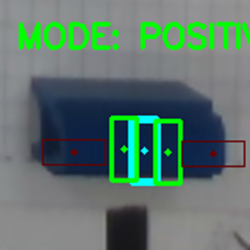
\includegraphics[width=0.2\textwidth]{Figures/chapter4/Grasping/i_gt.png} & 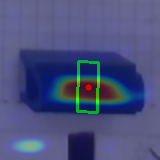
\includegraphics[width=0.2\textwidth]{Figures/chapter4/Grasping/i_resnet.png} & 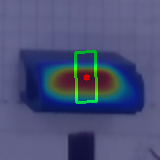
\includegraphics[width=0.2\textwidth]{Figures/chapter4/Grasping/i_swin.png} \\
\hline
L-shape & 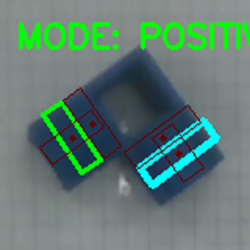
\includegraphics[width=0.2\textwidth]{Figures/chapter4/Grasping/l_gt.png} & 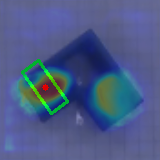
\includegraphics[width=0.2\textwidth]{Figures/chapter4/Grasping/l_resnet.png} & 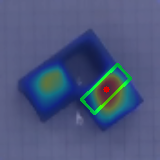
\includegraphics[width=0.2\textwidth]{Figures/chapter4/Grasping/l_swin.png} \\
\hline
T-shape & 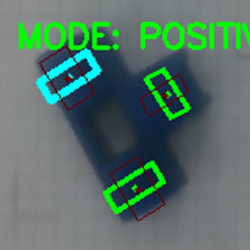
\includegraphics[width=0.2\textwidth]{Figures/chapter4/Grasping/t_gt.png} & 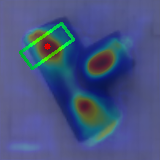
\includegraphics[width=0.2\textwidth]{Figures/chapter4/Grasping/t_resnet.png} & 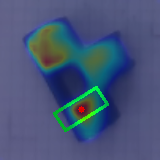
\includegraphics[width=0.2\textwidth]{Figures/chapter4/Grasping/t_swin.png} \\
\hline
\end{tabular}
\end{table}

\paragraph{Model Selection (ResNet-UNet vs Swin Transformer)}

Based on both quantitative and qualitative evaluation, ResNet-UNet was selected as the final grasp prediction model for deployment. Quantitatively, ResNet-UNet achieved a lower best validation loss compared to the Swin Transformer model, which indicates better overall agreement with the supervision signals (grasp quality and grasp orientation, including the negative-grasp penalties). In addition, ResNet-UNet reached a higher Top-1 validation performance and converged more stably under the same training settings.

Qualitatively, ResNet-UNet produced more localized and sharper high-confidence grasp regions, leading to more consistent grasp center placement on the object body. In contrast, Swin Transformer predictions were often more diffuse (smoother confidence maps) and sometimes exhibited multiple competing peaks. While this behavior can reflect modeling uncertainty and the existence of multiple feasible grasps, it may also increase the chance that the Top-1 selected grasp lies closer to object edges, which is undesirable for reliable execution.

A plausible explanation for the observed performance gap is that CNN encoder-decoder architectures provide a strong inductive bias for pixel-level localization, which is particularly beneficial in dense prediction tasks with limited training data. In our setting, the dataset size is relatively small (cropped brick images), and the task requires precise spatial alignment between image features and grasp targets. Transformers, including Swin, typically excel when sufficient data is available to learn robust attention patterns and higher-level representations. Therefore, it is likely that the Swin Transformer model would benefit from larger-scale training data, stronger pretraining aligned with the input modality (RGB-D), and/or more extensive hyperparameter tuning.

For these reasons, ResNet-UNet was chosen as the primary model for the project due to its better generalization, more reliable localization, and more stable qualitative behavior on the grasping task.
